\section{Results} \label{sec:results}
We present the posterior distributions of the DEM parameters for the SIMBA
(orange), TNG (blue), and EAGLE (green) hydro simulations in
Figure~\ref{fig:abc}. The DEM parameters include $\mtaum$, $\mtaus$, and
$\ctau$, which parameterize the $M_*$ dependence, $\sfr$ dependence, and 
amplitude of $\tau_V$, the $V$-band optical depth. $\tau_V$ dictates the
overall strength of the dust attenuation. They also include $\mdeltam$,
$\mdeltas$, and $\cdelta$, which parameterize the $M_*$ dependence, $\sfr$ dependence,
and amplitude of $\delta$, the slope offset of the attenuation curve
(Section~\ref{sec:dem} and Table~\ref{tab:free_param}). The posteriors 
are derived using ABC (Section~\ref{sec:abc}) and the contours mark the 
$68\%$ and $95\%$ confidence intervals. 

In addition, we also present the observables derived from median of the DEM
posteriors for the SIMBA (orange), TNG (blue), and EAGLE (green) simulations 
in Figure~\ref{fig:dem}. We include the observables for SDSS in the left-most 
panel for comparison (Section~\ref{sec:obs}). The top panels present the $(G-R) - M_r$ 
color-magnitude relations while the bottom panels present the $(FUV-NUV) - M_r$
relations. In Figure~\ref{fig:obs}, where we compare of the same observables
but for simulations without any dust prescription, we find dramatic differences 
in observable-space between SDSS and the simulations. In contrast, {\em using
DEMs we produce $(G-R) - M_r$ and $(FUV-NUV) - M_r$ relations consistent with
SDSS for all of the simulations}. 

The agreement in the observables is inspite of the significant differences 
in the SMFs and $M_*$-SFR relations (Figures~\ref{fig:smfs} and~\ref{fig:msfr}). 
In other words, the DEM has the flexiblity to reproduce observations even for 
simulations that predict galaxy populations with significantly different
physical properties. We emphasize that the DEM is based on the standard
prescriptions for dust attenuation and, thus, serve as a flexible
parameterization within the bounds of our current understanding of dust in galaxies.

Figure~\ref{fig:dem} highlights two key points. First, any comparison of
simulations must account for dust. Dust entirely changes the predictions of
simulations in observables-space. Fortunately, the DEM provides a simple framework
for including dust without the need for expensive ray-tracing methods. 
Second, the current limiations in our understanding of dust in galaxies 
significant impedes our ability to understand galaxy formation from simulations. 
To robustly interpret any comparison of simulations, we would need to
marginalize over dust (\emph{e.g.} DEM parameters). Since DEMs can produce
consistent observables for a range of simulations, marginalizing over dust
would leave little constraining power on the subgrid prescriptions (\emph{i.e.}
galaxy physics) of the simulations. 

While DEMs demonstrate that dust is a major bottleneck for interpreting galaxy
simulations, they also provide some insights into dust. For instance, the
posteriors of DEM parameters in Figure~\ref{fig:abc} reveal consistent trends
among the simulations. In all three simulations, we find significant positive
$M_*$ dependence of $\tau_V$: $\mtaum \sim 2$. Galaxies with higher $M_*$ have
overall higher dust attenuation. 
\ch{how does this compare to the literature?} 

We also find overall little $M_*$ and ${\rm SFR}$ dependence in $\delta$. In
fact, the amplitude of $\delta$ is roughly consistent with 0.  
\ch{what does this mean?}
\ch{how does this compare to the literature?} 
This is consistent with \cite{salim2020}, where they measured the attenuation
curve slopes of $23,000$ galaxies from GALEX-SDSS-WISE Legacy Catalog 2
(\ch{cite}). 

paragraph on the variation of attenuation curves based on 
\ch{what does this mean?}
While an empirical prescription like DEM doesn't allow explicit modeling of the
complex dust-star geometry, it does a good job at mimicking it. 
\ch{how does this compare to the literature?} 
comparison to \cite{narayanan2018} paper 

paragraph on restating how we can learn about dust through DEMs based on trends we see
across all simulations. summarize main findings again. 

\ch{What do the differences in DEM parameters say about the differences among
the hydro sims?} 
The whole SIMBA discrepancy
\ch{combining our understanding of dust maybe we can glean something about
galaxy evolution}

\begin{figure}
\begin{center}
    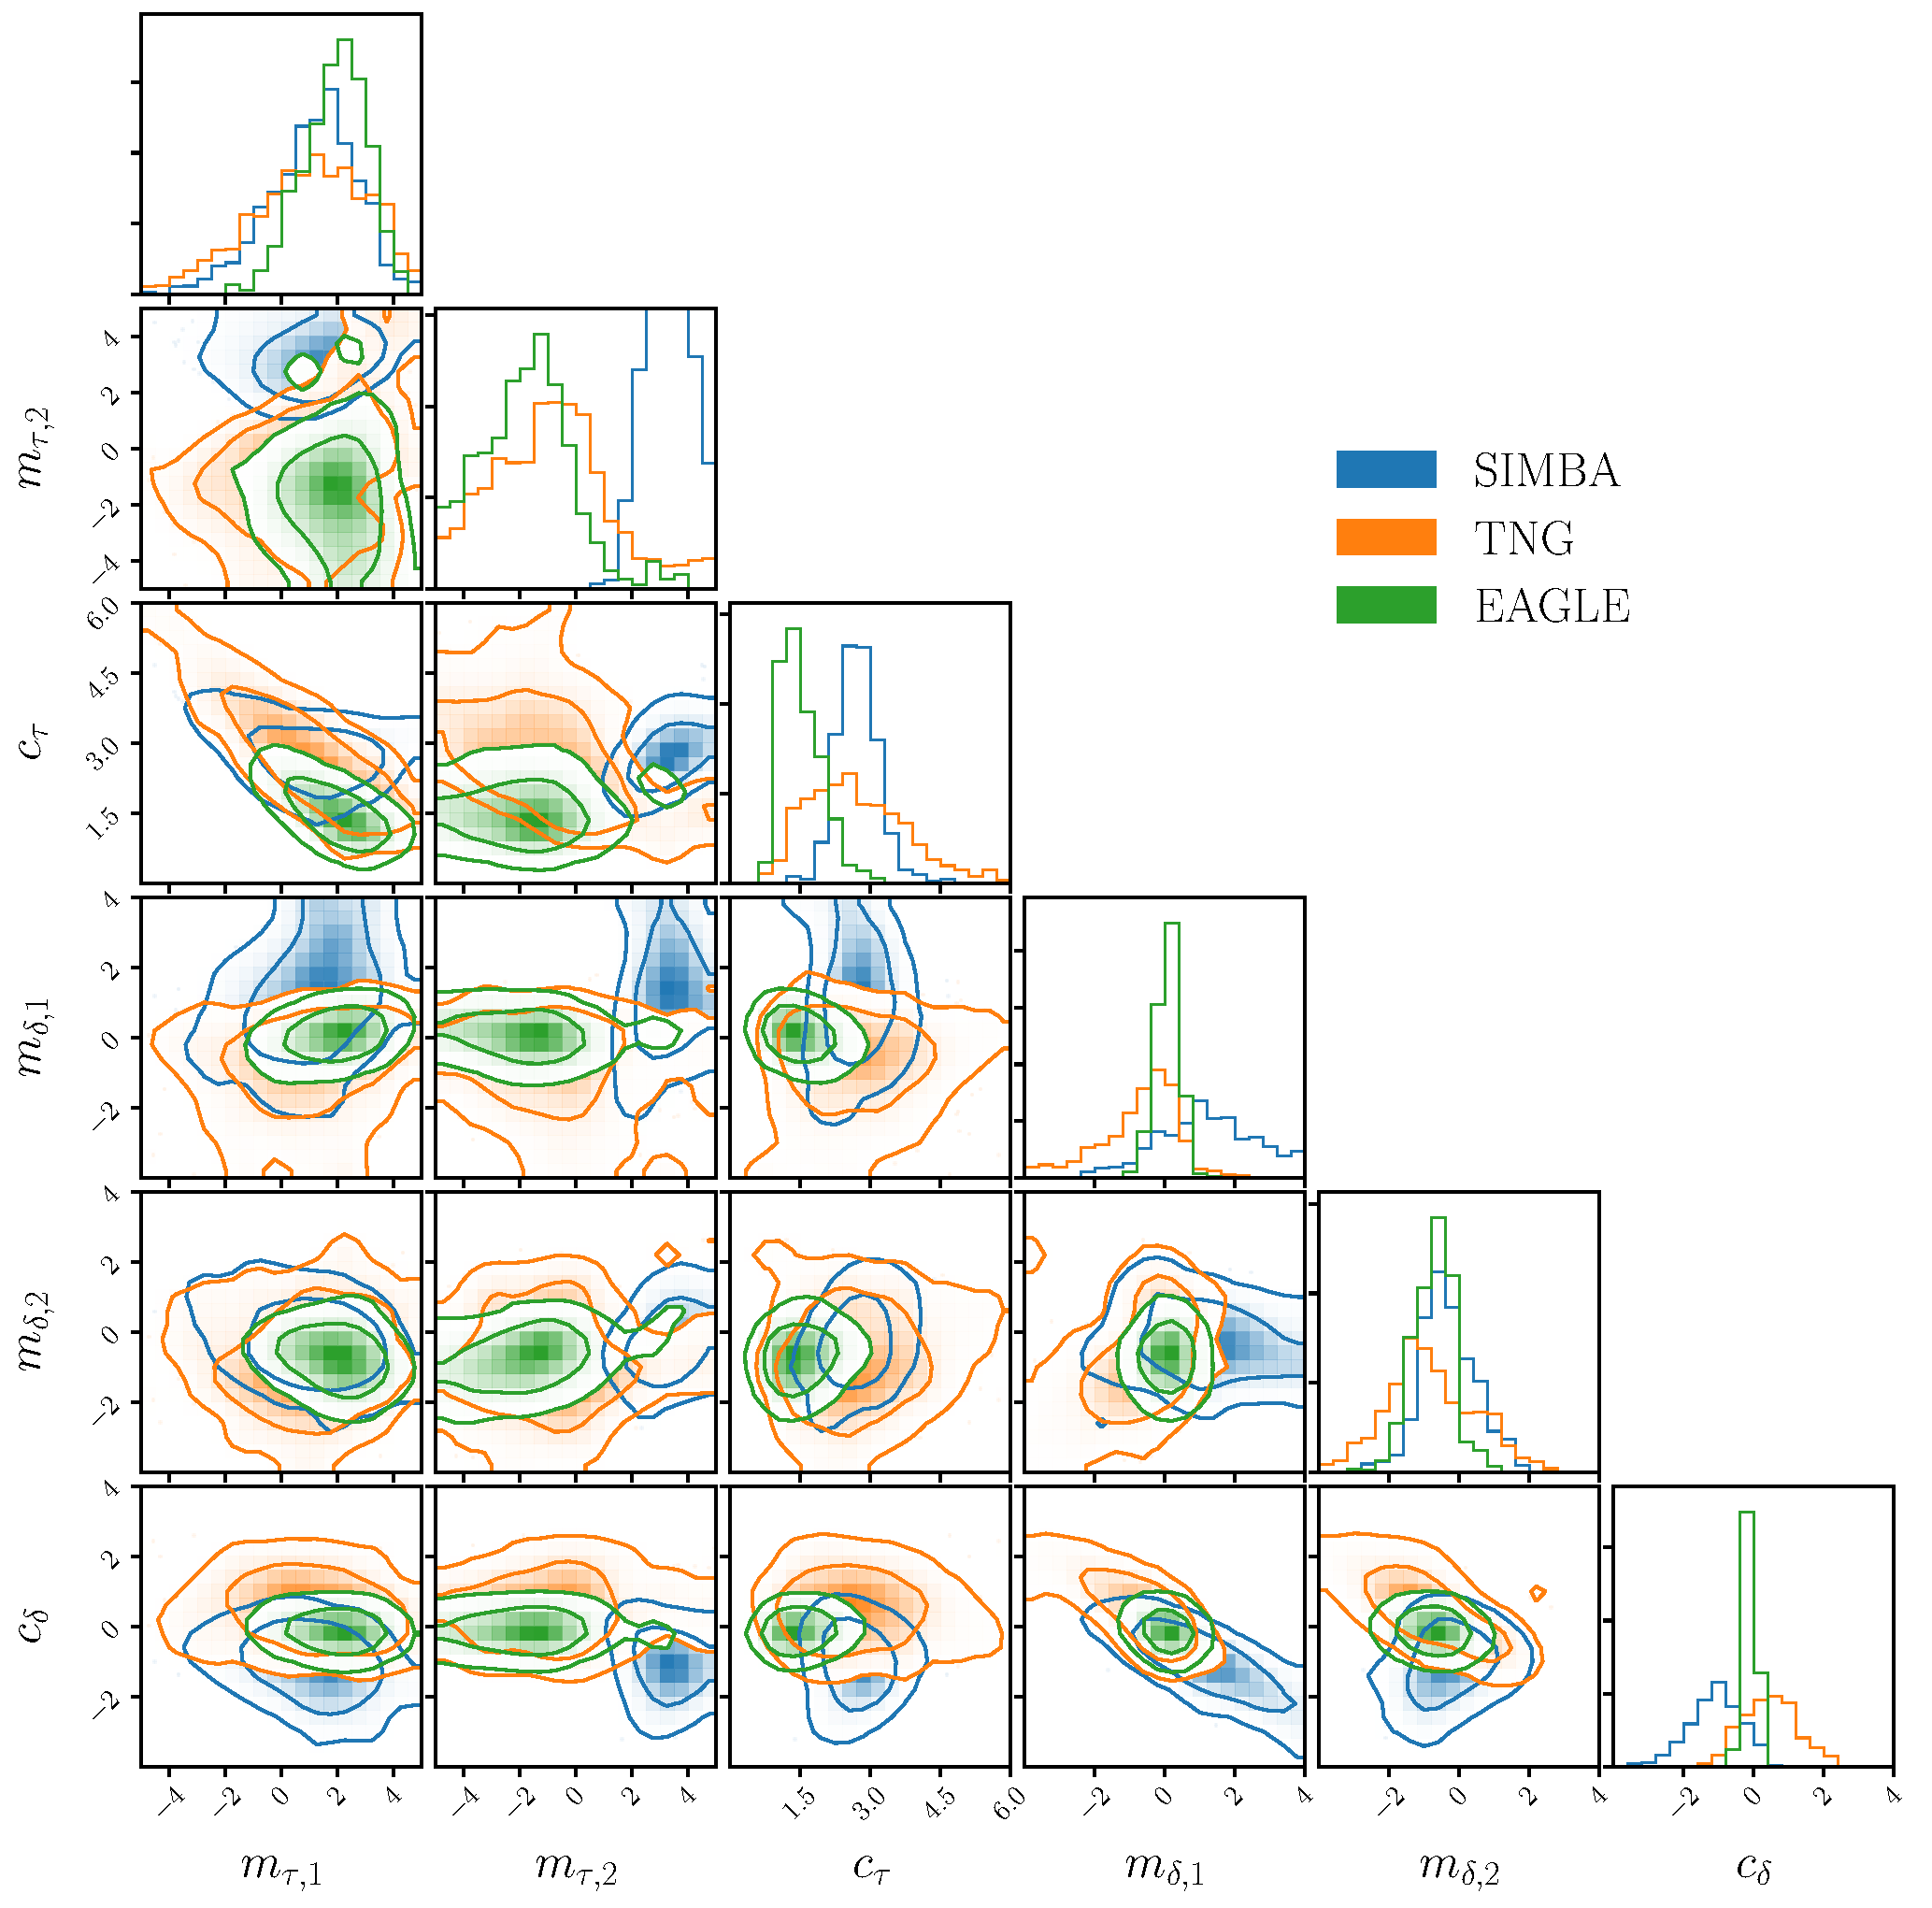
\includegraphics[width=\textwidth]{figs/abc.pdf}
    \caption{\label{fig:abc}
    Posterior distributions of our DEM parameters for the SIMBA (orange), TNG
    (blue), and EAGLE (green) hydro simulations. The contours mark the $68\%$
    and $95\%$ confidence intervals. We derive these posteriors using
    Approximate Bayesian Computation (ABC, Section~\ref{sec:abc}) and describe
    the parameters in Section~\ref{sec:dem} and Table~\ref{tab:free_param}. 
    In all simulations, dust attenuation increases for higher $M_*$ galaxies 
    ($m_{\tau,M_*} \sim 2$). The simulations also have consistent optical 
    depth amplitudes ($c_\tau$). However, the ${\rm SFR}$ dependence of
    $\tau_V$ is different among the simulations. For TNG and EAGLE,
    star-forming galaxies have lower $\tau_V$; for SIMBA quiescent galaxies
    have lower $\tau_V$. Meanwhile, for the slope offset of the attenuation
    curve, $\delta$, we find little $M_*$ and ${\rm SFR}$ dependence in the
    simulations and that the amplitude ($c_\tau$) is consistent with 0. 
    }
\end{center}
\end{figure}

\begin{figure}
\begin{center}
    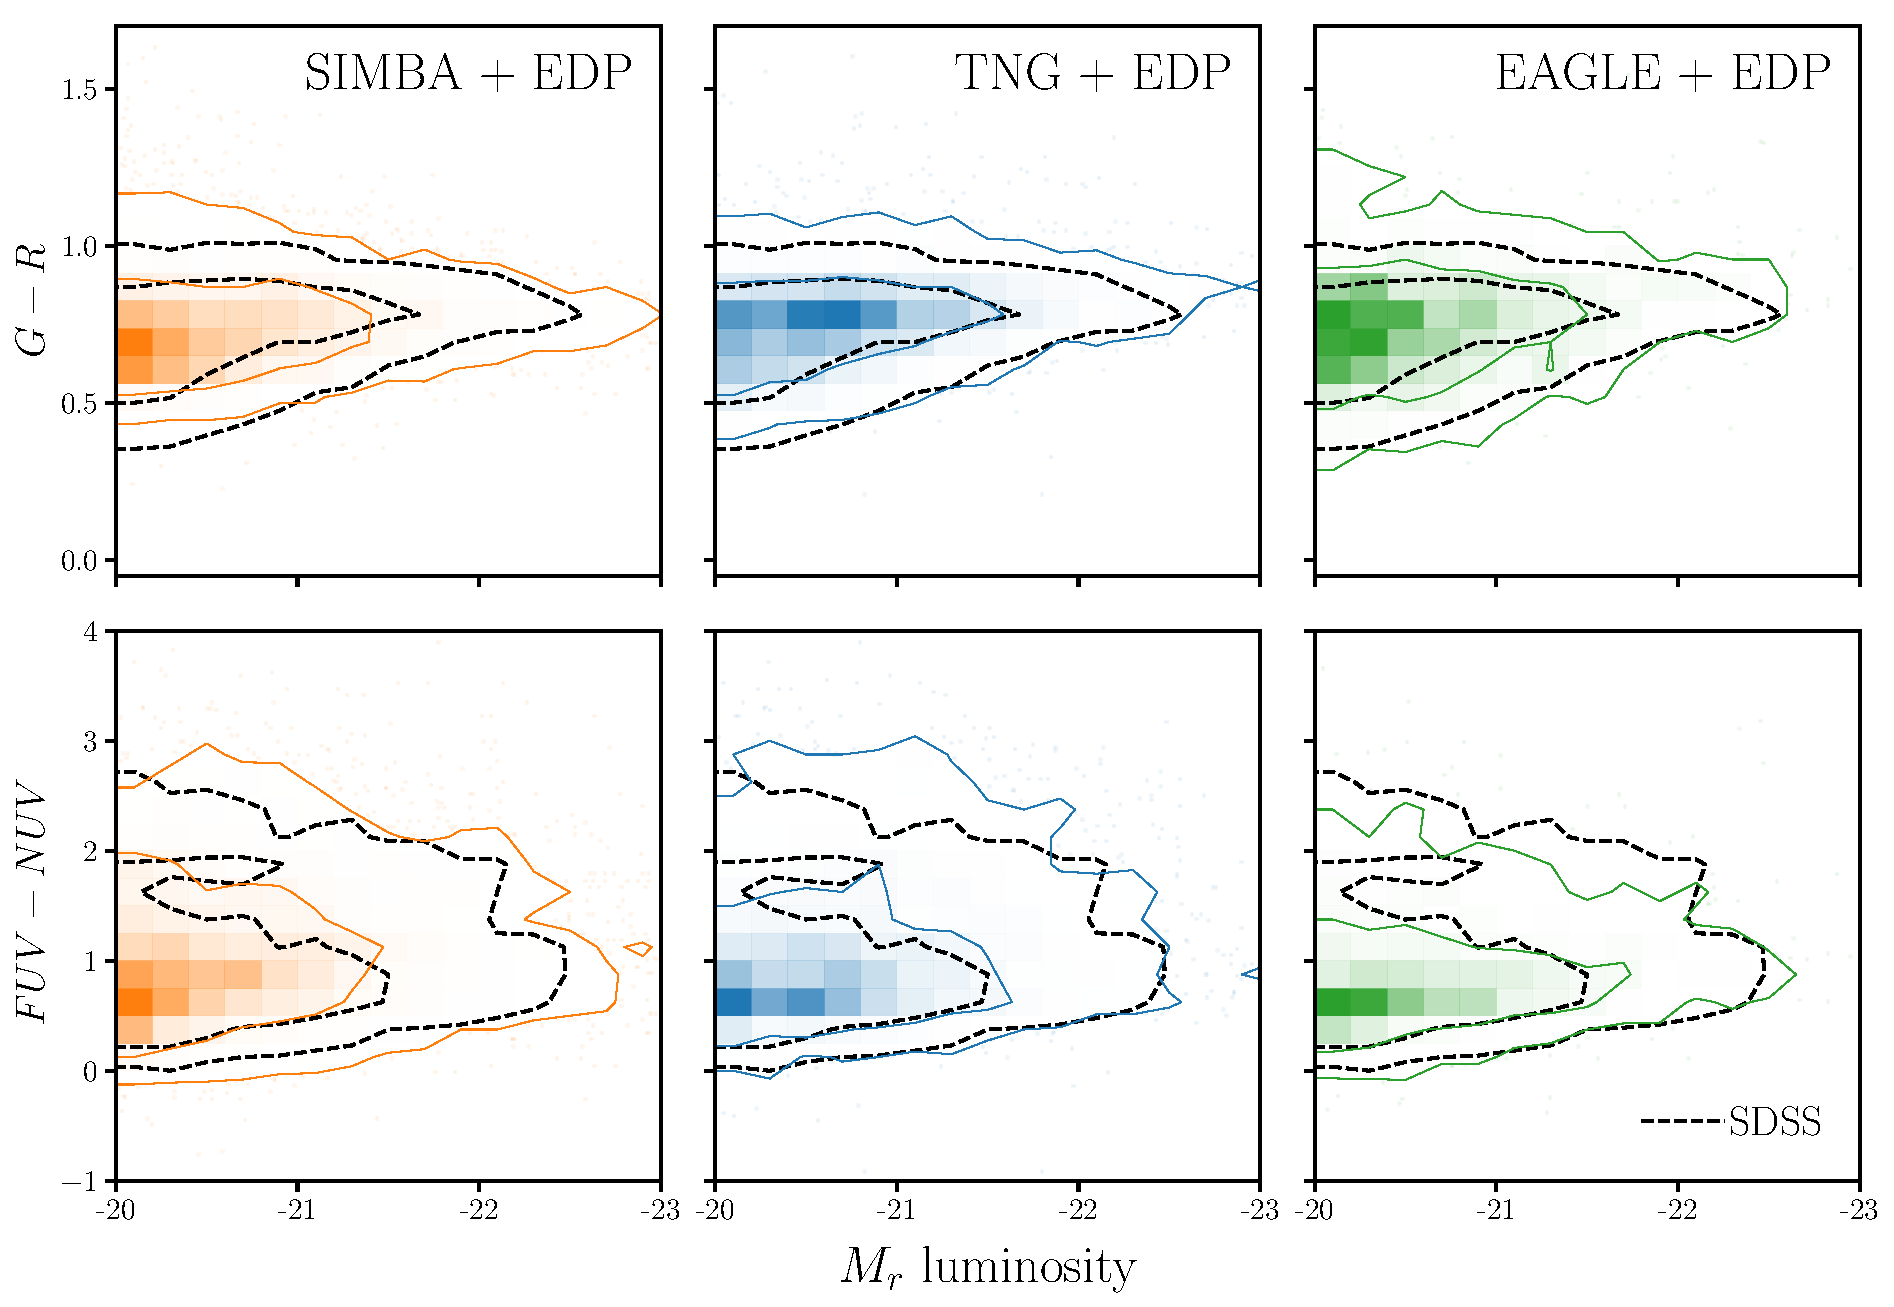
\includegraphics[width=\textwidth]{figs/abc_observables.pdf}
    \caption{\label{fig:dem}
    $(G-R) - M_r$ color-magnitude (top panels) and $(FUV-NUV) - M_r$ (bottom
    panels) relations predicted by the median DEM posteriors for the SIMBA
    (orange), TNG (blue), and EAGLE (green) hydro simulations. For comparison, 
    we include the observables for SDSS in the left-most panel
    (Section~\ref{sec:obs}). The median posterior DEMs produce dramatically 
    different observables than when we do not include any dust prescription
    (Figure~\ref{fig:obs}). Hence, dust must be account for when interpreting 
    and comparing simulations. Moreover, with the DEMs, all three simulations
    produce observables consistent with SDSS. Since different simulations can 
    produce reproduce observations by varying dust, dust significantly limits
    our ability to constrain the physical processes that go into galaxy
    simulations. 
    }
\end{center}
\end{figure}

\ch{More detailed look into the DEM observables.}
\begin{itemize}
    \item how does it compare to EAGLE+SKIRT? 
\end{itemize}
What are the limitations of DEM and how can it be improved? 
\begin{itemize}
    \item too many luminous galaxies
    \item color distribution isnt' perfect. 
    \item There isn't a whole lot of flexibility for SFR=0 galaxies predicted by
    simulations and they do not agree well with observations \ref{sec:res}. 
\end{itemize}


\begin{figure}
\begin{center}
    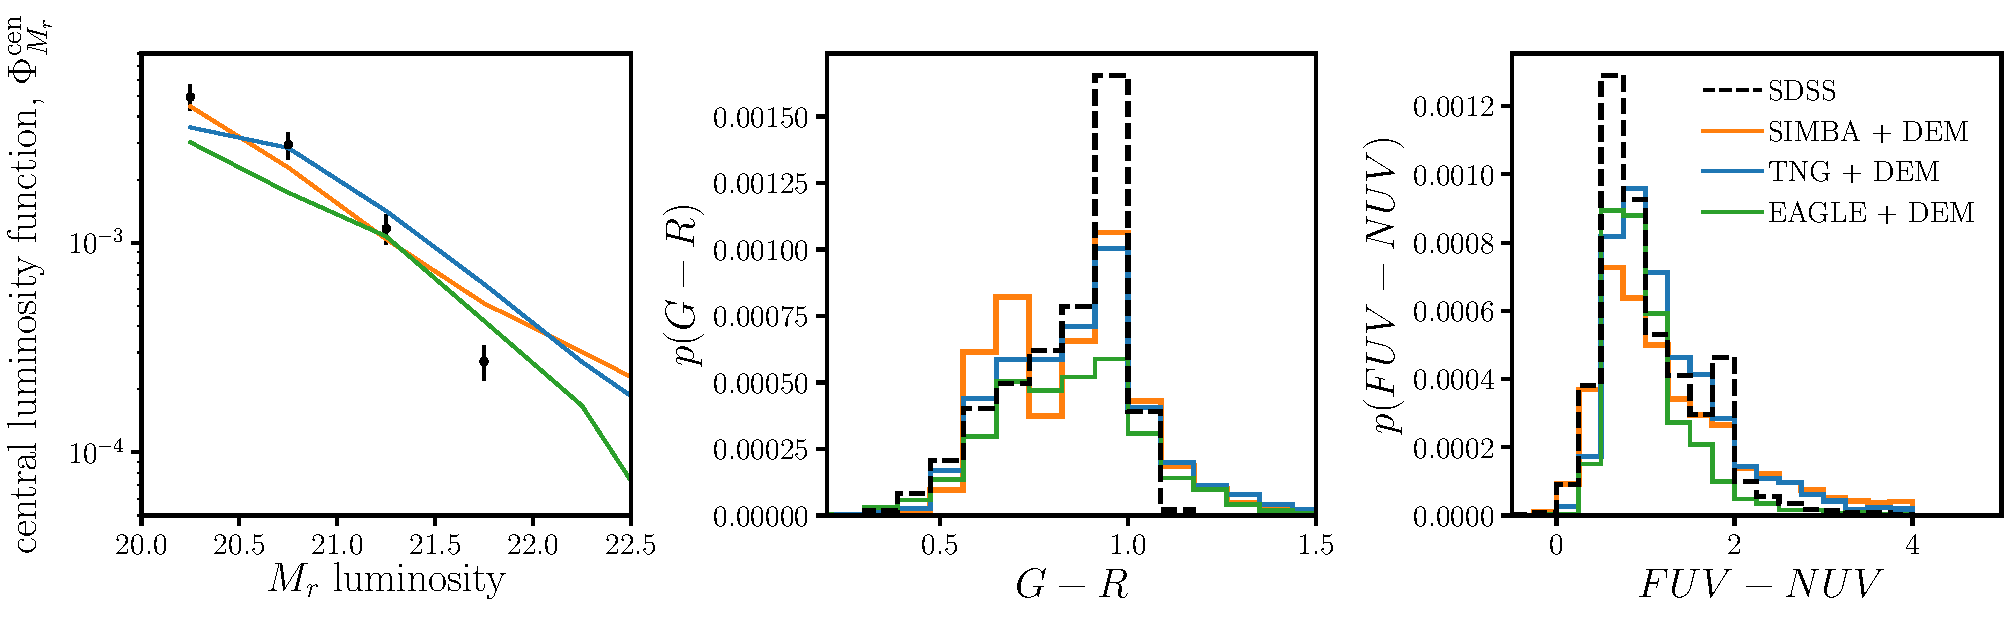
\includegraphics[width=\textwidth]{figs/abc_observables_1d.pdf}
    \caption{Comparison of the observables predicted by the simulations with
    the posterior DEM.}
\label{fig:dem1d}
\end{center}
\end{figure}

\ch{How robust are our results?}
We fix the UV bump to reduce the number of parameters. But when run our
analysis without fixing the UV bump, we find it does not impact our results.
We also get no constraints on the UV bump parameters. 

We rely on the slab model. But nothing changes when we use a more flexible
truncated normal distribution in Appendix~\ref{sec:nonslab}. tnorm DEM model allows us to also vary the
scatter of the attenuation curve 

\ch{How about our prior choice?}
%\begin{figure}
%\begin{center}
%    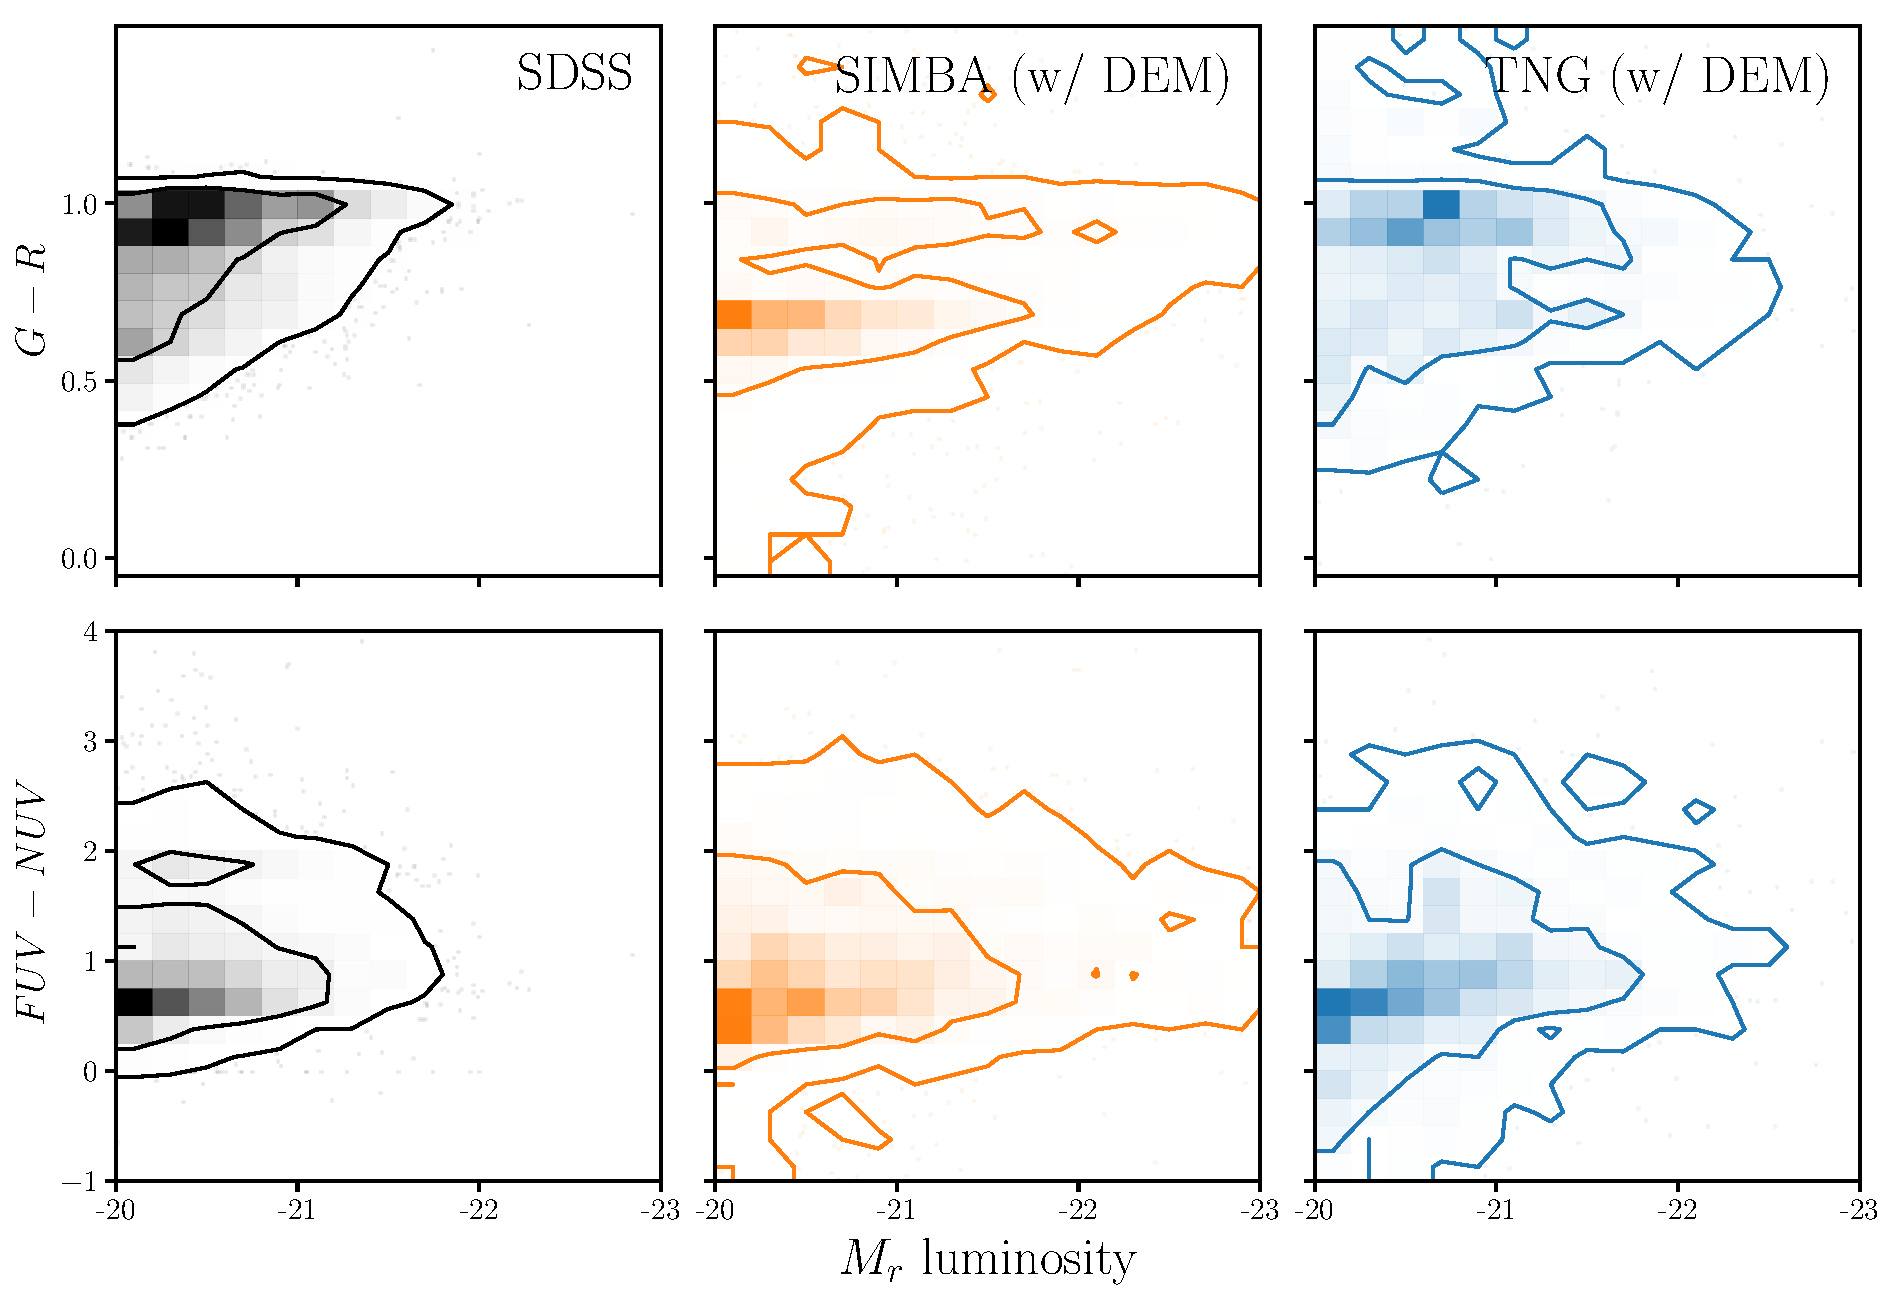
\includegraphics[width=\textwidth]{figs/abc_tnorm_observables.pdf}
%    \caption{Comparison of the observables predicted by the simulations with
%    the posterior DEM.}
%\label{fig:dem}
%\end{center}
%\end{figure}

\ch{If we marginalize over dust, can we learn anything about galaxy evolution
from the simulation?}

Are there observables that hydro sims + DEMs cannot reproduce? What does that say about the hydro sims?

What observables are unaffected by DEMs? We should chase those observables. 

We clearly have to becareful with overinterpreting hydro sims because modifying
dust allows us to reproduce whatever we want. 
\begin{itemize}
    \item Should we bother calibrating our empirical and semi-analytic models
        to hydrodynamic simulations when the hydro sims also require
        marginalizing over dust parameters? Does this mean that if our goal is
        to make realistic mocks, we can be relatively careless about 
\end{itemize}


\ch{What are some applications for DEMs?}
Realistic mock catalogs that reproduce observations in observable-space rather
than physical parameter space.  

%\begin{figure}
%\begin{center}
%    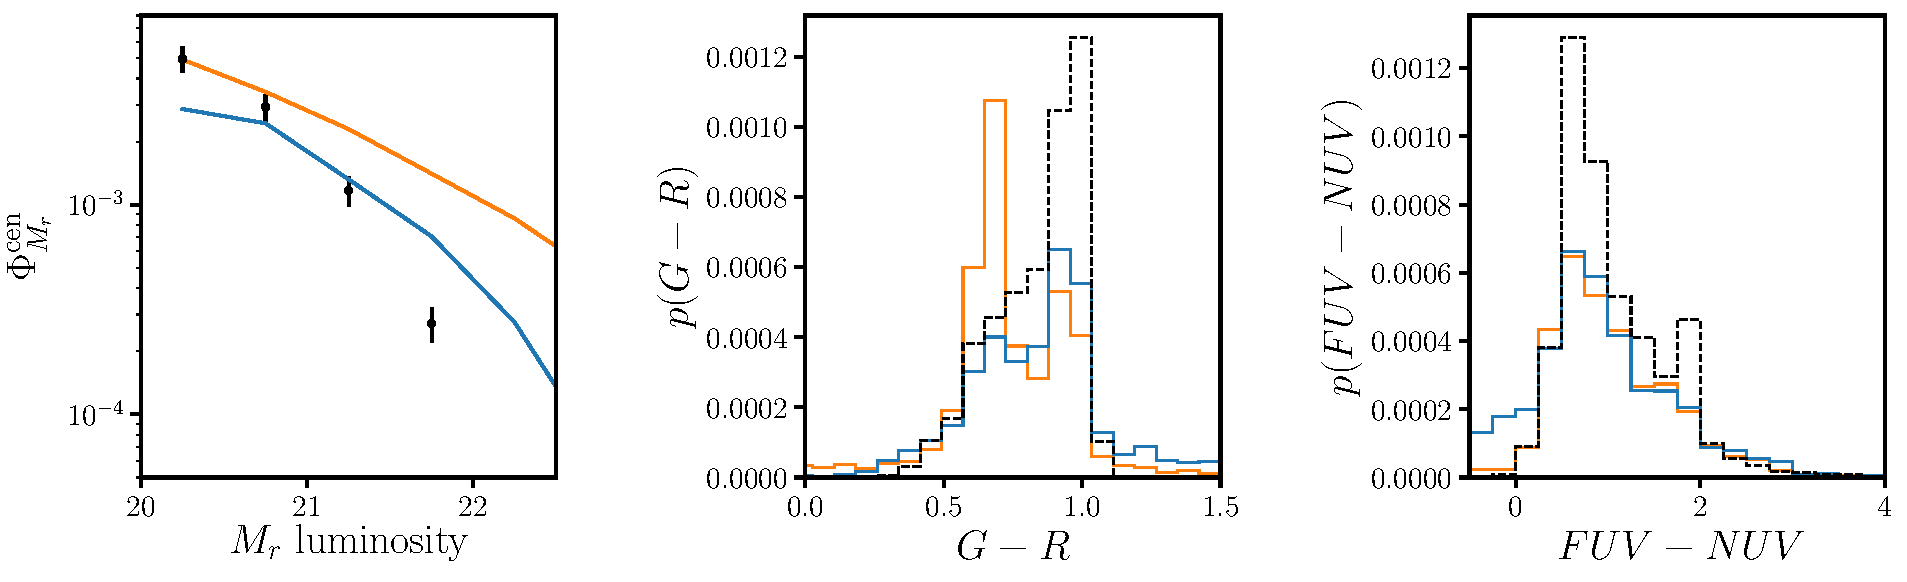
\includegraphics[width=\textwidth]{figs/abc_tnorm_observables_1d.pdf}
%    \caption{Comparison of the observables predicted by the simulations with
%    the posterior DEM.}
%\label{fig:dem}
%\end{center}
%\end{figure}
